\documentclass[11pt,aspectratio=169]{beamer}
\usetheme{Copenhagen}

\AtBeginSection[]{
  \begin{frame}
  \vfill
  \centering
  \begin{beamercolorbox}[sep=8pt,center,shadow=true,rounded=true]{title}
    \usebeamerfont{title}\insertsectionhead\par%
  \end{beamercolorbox}
  \vfill
  \end{frame}
}

\usepackage{amsmath}
\usepackage{amssymb}
\usepackage{bm}
\usepackage{amsthm}
\usepackage{enumerate}
\usepackage{graphicx}
\usepackage{psfrag}
\usepackage{color}
\usepackage{url}
\usepackage{listings}
\usepackage{xcolor}
\usepackage{tikz}
% \usetikzlibrary{positioning}
% \tikzset{main node/.style={circle,fill=gray!20,draw,minimum size=.5cm,inner sep=0pt},}

% \definecolor{codegreen}{rgb}{0,0.5,0}
% \definecolor{codewhite}{rgb}{1,1,1}
% \definecolor{codegray}{rgb}{0.5,0.5,0.5}
% \definecolor{codepurple}{rgb}{0.58,0,0.82}
% \definecolor{codeblack}{rgb}{0,0,0}
% \definecolor{codeorange}{rgb}{0.8,0.4,0}

% \lstdefinestyle{mystyle}{
    % backgroundcolor=\color{codewhite},   
    % commentstyle=\color{codegray},
    % keywordstyle=\color{codegreen},
    % numberstyle=\color{codegray},
    % stringstyle=\color{codeorange},
    % basicstyle=\ttfamily ,
    % breakatwhitespace=false,         
    % breaklines=true,                 
    % captionpos=b,                    
    % keepspaces=true,                 
    % numbers=left,                    
    % numbersep=5pt,                  
    % showspaces=false,                
    % showstringspaces=false,
    % showtabs=false,                  
    % tabsize=4
% }
% \lstset{style=mystyle}


% \setlength{\hoffset}{-1in}
% \addtolength{\textwidth}{1.5in}
% \setlength{\voffset}{-1in}
% \addtolength{\textheight}{1.5in}
\newcommand{\be}{\begin{enumerate}}
\newcommand{\ee}{\end{enumerate}}
\newcommand{\BigO}[1]{\ensuremath\mathcal{O}\left(#1\right)}
\newcommand{\il}[1]{\lstinline!#1!}
\newcommand{\norm}[1]{\left|\left|#1\right|\right|}
\newcommand{\abs}[1]{\left|#1\right|}
\newcommand{\parens}[1]{\left(#1\right)}
\newcommand{\bracks}[1]{\left\{#1\right\}}
\newcommand{\sqbracks}[1]{\left[#1\right]}
\newcommand{\vep}{\varepsilon}
\newcommand{\ceiling}[1]{\left\lceil#1\right\rceil}
\newcommand{\R}{\mathbb{R}}
\newcommand{\N}{\mathbb{N}}
\newcommand{\Z}{\mathbb{Z}}
\newcommand{\F}{\mathbb{F}}
\newcommand{\C}{\mathbb{C}}
\newcommand{\A}{\mathcal{A}}
\newcommand{\hilbert}{\mathcal{H}}
\newcommand{\distrib}[2]{\text{#1}\left(#2\right)}
\newcommand{\dd}[2]{\frac{d#1}{d#2}}
\newcommand{\parshal}[2]{\frac{\partial#1}{\partial#2}}
\newcommand{\abracks}[1]{\left< #1\right>}
\newcommand{\nullspace}[1]{\text{null }#1}
\newcommand{\LT}[1]{\mathcal{L}\parens{#1}}
\newcommand{\poly}[2]{\mathcal{P}_{#1}\parens{#2}}
\newcommand{\cont}[3]{\mathcal{C}_{#1}^{#2}\parens{#3}}
\newcommand{\range}[1]{\text{range }#1}
\newcommand{\one}{\mathbbm{1}}

\title{A study on quantifying effective training of DLDMD}
\author{Joseph A.G. Diaz}
\institute{Master of Science in Applied Mathematics\\ 
           with a Concentration in Dynamical Systems,\\
           San Diego State University}
\date{\today}

\begin{document}

    \frame{\titlepage}

    \begin{frame}
        \frametitle{Introduction}

        In the study of dynamical systems a central problem is how to derive models 
        from measured data to facilitate the prediction of future states. The data-driven
        method Dynamic Mode Decomposition and it's extensions offer a compelling avenue
        in the problem of prediction from time-series data.

        The marriage of these methods with Machine Learning and Neural Networks allows for
        the leveraging the power of these tools in the space. 

        If standard metrics of model training are unavailable, 
    
    \end{frame}

    \begin{frame}
        \frametitle{Introduction - Koopmanism}
        We seek a predictive model for a time series 
        $\bracks{\boldsymbol{y}_j}_{j=1}^{N^T+1}$, which are the measurements of a 
        dynamical system of the form
        \begin{equation}
            \dd{\boldsymbol{y}}{t} = f\parens{\boldsymbol{y}(t)},\quad \boldsymbol{y}(0) 
            = \boldsymbol{x} \in \mathcal{M} \subseteq \R^{N_s}
        \end{equation}
        Denote $\boldsymbol{\varphi}(t;\boldsymbol{x}) =
        \boldsymbol{y}(t)$ to be the flow map from $\boldsymbol{x}$
        and $g: \mathcal{M} \to \C,$ be a square integrable 
        observable then, by \cite{koopman}, $\exists \mathcal{K}$ such that
        \begin{equation}
            \mathcal{K}^t g(\boldsymbol{x}) = g(\boldsymbol{\varphi}(t; \boldsymbol{x})),
        \end{equation}
        Finding the eigen-values $\bracks{\lambda_\ell}$ and 
        eigen-functions $\bracks{\boldsymbol{\phi}_\ell}$ of $\mathcal{K}$ yields
        \begin{equation}
            \mathcal{K}^t\boldsymbol{\phi}_\ell = \exp(t\lambda_\ell)\boldsymbol{\phi}
            _\ell \implies g(\boldsymbol{x}) = \sum_{\ell \in \N} a_\ell \boldsymbol{\phi}_
            \ell(\boldsymbol{x}),    
        \end{equation}
        A modal decomposition of $g$.

    
    \end{frame}

    \begin{frame}
        \frametitle{Introduction - DMD and EDMD}
        From here advancing the dynamics to time $t$ is equivalent to writing
        \begin{equation}
            \mathcal{K}^{t} g(\boldsymbol{x}) = \sum_{\ell \in \N} a_\ell 
            \exp(t\lambda_\ell)\boldsymbol{\phi}_\ell (\boldsymbol{x})
        \end{equation} 
        This is the basis of Dynamic Mode Decomposition (DMD). If we suppose 
        \begin{equation}
            g(\boldsymbol{x}) = \sum_{\ell = 1}^{N_O} a_\ell \boldsymbol{\psi}_\ell
            (\boldsymbol{x}) 
        \end{equation}
        with basis $\bracks{\boldsymbol{\psi}_\ell}_{\ell=1}^{N_O}$ of a subspace, 
        then applying $\mathcal{K}$ for discrete time implies that
        \begin{align} 
            \mathcal{K}^{\delta t} g(\boldsymbol{x}) &= \sum_{\ell = 1}^{N_O} a_\ell 
            \exp(\delta t\lambda_\ell)\boldsymbol{\psi}_\ell (\boldsymbol{x}) \\
            &= \sum_{\ell = 1}^{N_O} \boldsymbol{\psi}_\ell (\boldsymbol{x})
            (\boldsymbol{K}_O^T
            \boldsymbol{a})_\ell + r(\boldsymbol{x};\boldsymbol{K}_O)
        \end{align}
    \end{frame}

    \begin{frame}
        \frametitle{Introduction - Time advancement}
        Where
        \begin{equation}
            \boldsymbol{K}_O = \underset{K}{\text{argmin}}\norm{{\bf\Psi}_+ - K{\bf\Psi}_-}_F^2
        \end{equation}

        We define ${\bf\Psi}_\pm$ to be
        \begin{equation}
            {\bf\Psi}_- = \parens{\Psi_1\ \Psi_2\ \cdots \Psi_{N_T}},\quad {\bf\Psi}_+ = \parens{
            \Psi_2\ \Psi_3\ \cdots \Psi_{N_T+1}} 
        \end{equation}
        where $\bracks{\Psi_j}$ is an observable of the time series of interest 
        $\bracks{\boldsymbol{y}_j}$. What the expression for $\boldsymbol{K}_O$ tells 
        us is that, we are trying to find a one-step mapping from each data point
        to the next. Practically speaking, $\boldsymbol{K}_O$ is found
        %$\boldsymbol{K}_O$ approximates $\mathcal{K}$ for a one-step mapping and is found 
        using a singular value decomposition (SVD), with which we can write
        \begin{equation}
            {\bf\Psi}_- = {\bf U\Sigma W}^{\dagger} \implies \boldsymbol{K}_O = 
            {\bf\Psi}_+{\bf W\Sigma}^{-P}{\bf U}^{\dagger}
        \end{equation}
    \end{frame}

    \begin{frame}
        \frametitle{Introduction - Flow reconstruction}
        Finding the eigenvalues, eigenfunctions, and Koopman modes comes down to an 
        eigen-decomposition of $\boldsymbol{K}_O$,
        \begin{equation}
            \boldsymbol{K}_O = {\bf VTV}^{-1}, 
        \end{equation}
        with $\lambda_\ell = \ln(({\bf T})_{\ell\ell})/\delta t$,
        from which the dynamics can be approximated as 
        \begin{equation}
            y(t;\boldsymbol{x}) \approx \boldsymbol{K}_m\exp(t{\bf\Lambda}){\bf V}^{-1}\boldsymbol{\Psi}(\boldsymbol{x}) 
        \end{equation}
        where $\boldsymbol{\Psi}$ is the representation of the initial condition in terms of the observables, 
        $\boldsymbol{K}_m$ is the $N_S \times N_O$ matrix whose columns are the Koopman modes 
        $\bracks{{\bf k}_\ell}_{\ell=1}^{N_O}$ which solve the initial value problem
        \begin{equation}
            \boldsymbol{x} = \sum_{\ell=1}^{N_O}{\bf k}_\ell\boldsymbol{\phi}(\boldsymbol{x}),
        \end{equation}
        and ${\bf \Lambda}$ is the diagonal matrix whose elements are $\lambda_\ell
        = ({\bf \Lambda})_{\ell\ell}$.
    \end{frame}

    \begin{frame}
        \frametitle{Introduction - Neural Networks}
        Before we move on, a brief digression on Neural Networks (NNs) is appropriate. Ever since
        scientists discovered the relatively simple interaction between neurons and axons in 
        the human brain, they have been enamored with the ability to create a learning computer 
        with the similar ability to become more adept at a task with training and practice. 
        In the same way that art imitates life, the most straight-forward attempts have been 
        to construct artificial neural networks that pantomime the biological ones that we carry 
        around in our heads; and while these pale imitations have not been developed to rival the 
        human brain, they have led to some major achievements in automation. In much the same 
        way that a person is ``trained'' to perform a task by repeating it with feedback and 
        adjusting their performance as they go, an artificial NN uses data, a loss function, and 
        an optimization algorithm to change the state of the NN to one which can better accomplish 
        the task. The loss function and optimizer are to the feedback and behavioral adjustment 
        what the data is to the experience. 
    \end{frame}

    \begin{frame}
        \frametitle{Introduction - Function approximation and regression}
        Say we have a set of training data $d_{tr} = \bracks{(x_j, y_j)}_{j=1}^{N_{tr}}$ 
        and we believe that there is some function $f(x)$ such that 
        \begin{equation}
            y_j = f(x_j) + \vep_j,    
        \end{equation}
        where $\vep_j$ is assumed to be a sample drawn from $\mathcal{N}(0, \bar{\sigma}^2)$. 
        \cite{oreilly, theodoridis}
        Generally $f$ is not known; so we must, using the training data, build an estimator 
        $f_e(x; d_{tr})$ and measure the performance of the estimator by examining the quantity
        \begin{equation}
            \mathbb{E}_{d_{tr}}\sqbracks{\parens{f(x) + \vep - f_e(x;d_{tr})}^2} = 
            \text{bias}_{d_{tr}}^2 + \mathbb{V}(f_e) + \bar{\sigma}^2
        \end{equation}
        where 
        \begin{equation}
            \text{bias}_{d_{tr}} = \mathbb{E}_{d_{tr}}\sqbracks{f_e} - f(x)
        \end{equation}
        and 
        \begin{equation}
            \mathbb{V}(f_e) = \mathbb{E}_{d_{tr}}\sqbracks{\parens{\mathbb{E}_{d_{tr}}
            \sqbracks{f_e} - f_e(x; d_{tr})}^2}
        \end{equation}
        % With this framing, ML methods can be cast as attempts to find an estimator relative to
        % a given training set that balances the competing dilemmas of being too biased or allowing too
        % much variance. From the point of view of non-parametric statistics, we would need to utilize 
        % other techniques \cite{hollander} to determine the bias and variance of any given estimator. 
        For our purposes, 
        we will instead consider how metrics from information theory can be used to assess the change in 
        information as data is fed through a NN and a model is trained.
    \end{frame}

    \begin{frame}
        \frametitle{Introduction - DLDMD}
        The key innovation of 
        \cite{lago} is to use a neural network to come up with the collection of 
        observables on $\bracks{\boldsymbol{y}_j}$ that allow for the best prediction 
        of future system states, we call this method Deep Learning Enhanced DMD (DLDMD). 
        This is implemented by defining an encoder 
        $\mathcal{E}: \R^{N_S} \to \R^{N_O}$ and decoder $\mathcal{D}: \R^{N_O} \to \R^{N_S}$ composed of 
        dense layers such that 
        \begin{equation}
            (\mathcal{D}\circ\mathcal{E})(\boldsymbol{x}) = \boldsymbol{x}
        \end{equation}
        We choose $N_O \geq N_S$ and an appropriate loss function so that 
        $\mathcal{E}$ and $\mathcal{D}$ give a richer space of observables, called the 
        latent space, for EDMD to use when advancing the dynamics. The implementation 
        of NNs for this purpose requires a method of tuning to allow $\mathcal{E}$ and 
        $\mathcal{D}$ to learn the best representations possible. 
    \end{frame}
    
    \begin{frame}
        \frametitle{Introduction - The loss function}
        A natural choice
        considering these constraints is given by
        \begin{equation}
            \mathcal{L} = \alpha_1 \mathcal{L}_{\text{recon}} + \alpha_2 \mathcal{L}
            _{\text{dmd}} + \alpha_3 \mathcal{L}_{\text{pred}} +\alpha_4 
            \norm{\boldsymbol{W}_g}_2 \label{eqn:loss function} 
        \end{equation}
        where 
        \begin{align}
            \mathcal{L}_{\text{recon}} &= \frac{1}{N_T + 1}\sum_{j=1}^{N_T+1}\norm{\boldsymbol{y}_j - 
            (\mathcal{D}\circ\mathcal{E})(\boldsymbol{y}_j)}_2, \\
            \mathcal{L}_{\text{dmd}} &= E_r(\boldsymbol{K}_O), \\
            \mathcal{L}_{\text{pred}} &= \frac{1}{N_T}\sum_{j=1}^{N_T}\norm{\boldsymbol{y}_{j+1} - 
            \mathcal{D}\parens{VT^j V^{-1}\mathcal{E}(\boldsymbol{x})}}_2, \label{eqn:blah}
        \end{align}
        Recall that $N_T$ is the number of measurements in our time-series data after the first.
    \end{frame}

    \begin{frame}
        \frametitle{Introduction - The Network Architecture}
        Example of DLDMD newtork with $N_S = 2,\ N_O = 4,$ and $N_L = 3$ where every
        hidden layer has 16 neurons. The layers in the Figure are 
        labeled, sequentially, left to right: Enc in, Enc 0, Enc 1, Enc 2, Enc out, Dec in, 
        Dec 0, Dec 1, Dec 2, Dec out.
        \begin{figure}
            \centering
            \begin{minipage}{.5\textwidth}
                $$\mathcal{E}$$
                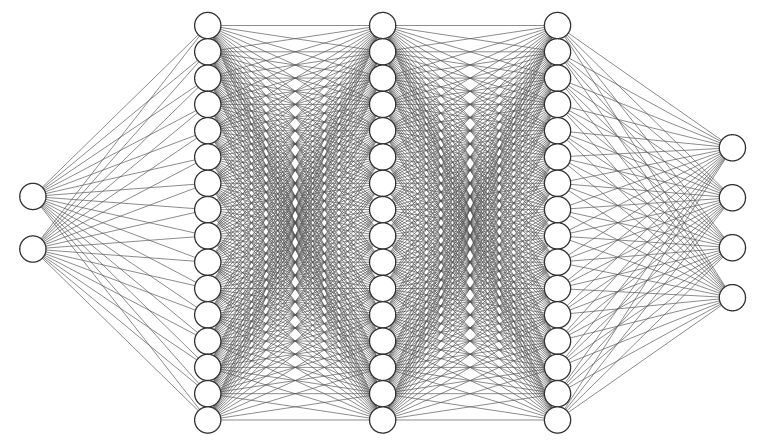
\includegraphics[width=\textwidth]{../Figures/Encoder.png}
            \end{minipage}%
            \begin{minipage}{.5\textwidth}
                $$\mathcal{D}$$
                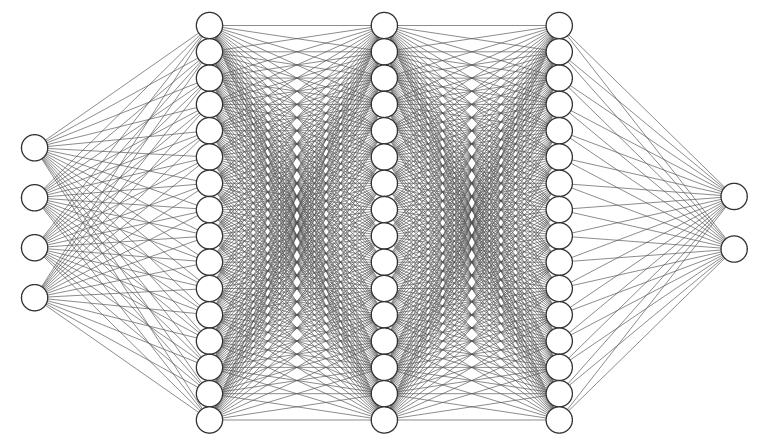
\includegraphics[width=\textwidth]{../Figures/Decoder.png}
            \end{minipage}
        \end{figure}
    \end{frame}

    \begin{frame}
        \frametitle{Introduction - The Dilemma}
        How can this be quantified? A useful starting point would be to examine the weights of
        the matrices that make up the layers of a model. For dense layers, passing a vector of 
        data $\boldsymbol{x} \in \R^{d}$ through a layer $L$ can be written as 
        \begin{equation}
            L(\boldsymbol{x}; {\bf A}, \sigma, {\bf b}) = \sigma({\bf A}\boldsymbol{x} + {\bf b})
        \end{equation}
        for some matrix ${\bf A} \in \R^{N_O\times d}$, vector ${\bf b} \in \R^{N_O}$ and (typically nonlinear)
        activation function $\sigma: \R^{N_O} \to \R^{N_O}$. For a given layer, $\sigma$ is a choice of the 
        model, but both ${\bf A}$ and ${\bf b}$ have entries that are tuned by the 
        optimizer as training takes places. The next state for each layer is dependent on the previous, so a reasonable 
        framing would be as one of a discrete dynamical system of the form
        \begin{equation}
            Q_{n+1} = P(Q_n)
        \end{equation}
        where $P$ is the training procedure and $Q_n$ represents the configuration of the network's
        weights at each epoch $n$. The initial state $Q_0$ is random with it's weights being
        selected from a probability distribution. 
    \end{frame}

    \begin{frame}
        \frametitle{Introduction - Information Theory}
        In the interest of examining 
        convergences, one might consider the following limit 
        \begin{equation}
            \lim_{n\to\infty} \norm{Q_{n+1} - Q_n}_2    
        \end{equation}
        for some two-norm on the space that $Q_n$ inhabits. While this ``one-step'' Cauchy 
        convergence will tell us whether the machine is approaching a particular configuration
        point-wise, this might not actually tell us much of anything else. The changes between 
        epochs is, in some sense, stochastic due to not knowing how the optimizer will update $Q$
        between epochs. As such, we propose a more statistical approach wherein we examine how the
        information content is changing from epoch to epoch. From the stochastic nature of the 
        evolution, we consider the entries of ${\bf A}$ and ${\bf b}$ for each layer to be drawn from a continuous 
        probability distribution $X$ and examine how it changes epoch to epoch.
    \end{frame}

    \begin{frame}
        \frametitle{Kullback-Leibler Divergence - Entropy}
        A measure of the uncertainty was 
        proposed in 1948 and this measure is known as \emph{informational entropy} \cite{shannon}
        or, simply, entropy. For a
        continuous distribution with density function $f(x)$, the entropy is given by 
        \begin{equation}
            h[f] = \mathbb{E}\sqbracks{-\log(f(x))} = -\int_X f(x)\log(f(x))\ dx    
        \end{equation}
        For the normally distributed $X$ defined above, we have the probability density function
        \begin{equation}
        f(x) = \frac{1}{\sigma\sqrt{2\pi}}\exp\parens{-\frac{1}{2}\parens{\frac{x-\mu}{\sigma}}^2} 
        \label{eqn:normal} 
        \end{equation}
        and the entropy integral for this evaluates to
        \begin{equation}
            h[f] = \frac{1}{2}\parens{\log(2\pi\sigma^2) + 1}
        \end{equation}
        which only depends on the variance.
    \end{frame}

    \begin{frame}
        \frametitle{Kullback-Leibler Divergence - Entropy example}
        \begin{figure}
            \centering
            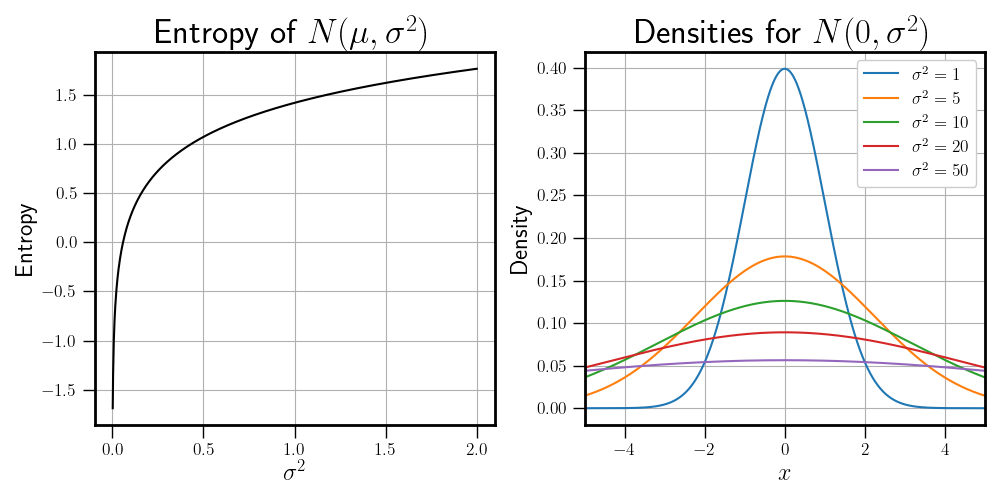
\includegraphics[width=\textwidth]{../Figures/entropy_densities_example.png}
        \end{figure}
    \end{frame}

    \begin{frame}
        \frametitle{Kullback-Leibler Divergence - Basic Definitions}
        The Kullback-Leibler Divergence (KLD) is a statistical distance between a 
        pair of probability distributions which measures how different a distribution $P$ is 
        from a reference distribution $Q$. A simple interpretation of the 
        divergence of $P$ from $Q$ is the expected excess surprise from using $Q$ as a model 
        when the actual distribution is $P$ \cite{kullback}. If $P$ and $Q$ are discrete distributions 
        defined on the probability space $X$, then the KLD of $P$ with 
        respect to $Q$ is given by
        \begin{equation}
            D_{KL}(P\ |\!|\ Q) = \sum_{x \in X}P(x)\log\parens{P(x)/Q(x)} \label{eqn:discrete KLD}
        \end{equation}
        In our cases, we are be dealing with a continuous random variable
        with probability density functions $p$ and $q$, for which the corresponding KLD formula 
        is
        \begin{equation}
            D_{KL}(P\ |\!|\ Q) = \int_X p(x)\log\parens{p(x)/q(x)}\ dx \label{eqn:continuous KLD}
        \end{equation}
    \end{frame}

    \begin{frame}
        \frametitle{Kullback-Leibler Divergence - Statistical Distance}
        The reason we can consider this a ``distance'' is that the KLD 
        is non-negative, $D_{KL}(P\ |\!|\ Q) \geq 0$, which is known as Gibbs 
        inequality and only equals 0 when $P = Q$ almost everywhere. As such, the distance
        between $P$ and $Q$ is 0 when they are the ``same'' distribution and some positive 
        number if they differ. For example, consider the random variables $X_1 \sim 
        \mathcal{N}(\mu_1, \sigma_1^2)$ and $X_2 \sim \mathcal{N}(\mu_2, \sigma_2^2)$ 
        with corresponding density functions given by equation \ref{eqn:normal}; the divergence 
        between the distributions is
        \begin{equation}
            D_{KL}(p\ |\!|\ q) = \frac{1}{2}\parens{\ln\parens{\frac{\sigma_2^2}{\sigma_1^2}} + 
            \frac{\sigma_1^2}{\sigma_2^2} + \frac{(\mu_1 - \mu_2)^2}{\sigma_2^2} - 1}, \label{eqn:normal divergence}
        \end{equation}
        Letting $\mu_1 = \mu_2$, $\sigma_1^2 = 1$, and allowing $\sigma_2^2$ to vary, we can 
        write 
        \begin{equation}
            D_{KL}(p\ |\!|\ q) = \frac{1}{2}\parens{\ln\sigma_2^2 + 
            \frac{1}{\sigma_2^2} - 1}, \label{eqn:normal divergence2}
        \end{equation}
    \end{frame}

    \begin{frame}
        \frametitle{Kullback-Leibler Divergence - normal distribution example}
        \begin{figure}
            \centering
            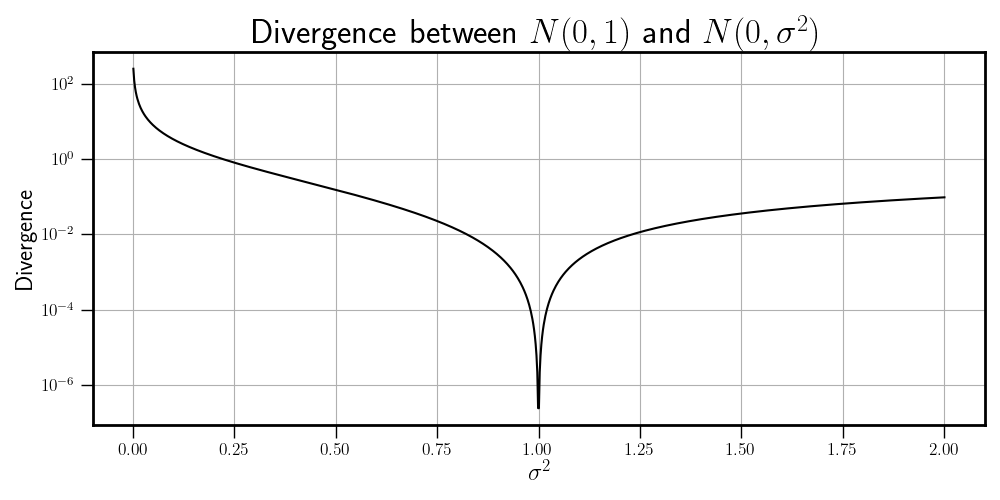
\includegraphics[width=\textwidth]{../Figures/divergence_example.png}
        \end{figure}
    \end{frame}

    \begin{frame}
        \frametitle{Kullback-Leibler Divergence - Kernel Density Estimation}
        The most 
        basic idea behind KDE is using a bin centering method and a smoothing factor, 
        called a kernel, to approximate a probability density $f$ from measured data in the form 
        of a histogram. This is accomplished with the \emph{kernel density estimator} for $f$
        given by
        \begin{equation}
            \hat{f}(x; K, h) = \frac{1}{nh}\sum_{i = 1}^n K\parens{\frac{x - x_i}{h}},
        \end{equation}
        where $K$ is the chosen kernel, $h$ is what's called the bandwidth parameter, and 
        $\{x_i\}_{i=1}^n$ is the data that generates our histogram. Per Epanechnikov, 
        the choice of kernel does not provide much statistical significance \cite{epanechnikov}; 
        but the choice of the bandwidth parameter $h$ is very crucial for finding a density estimate
        that approximates the underlying density function appropriately and can be thought of as an 
        analogue of the bin width for the affliated histogram. We choose $h$ using the 
        Improved Sheather-Jones algorithm \cite{botev}, which algorithmically finds an optimal 
        bandwidth using the data itself.
    \end{frame}

    \begin{frame}
        \frametitle{Kullback-Leibler Divergence - KDE example}
        \begin{figure}
            \centering
            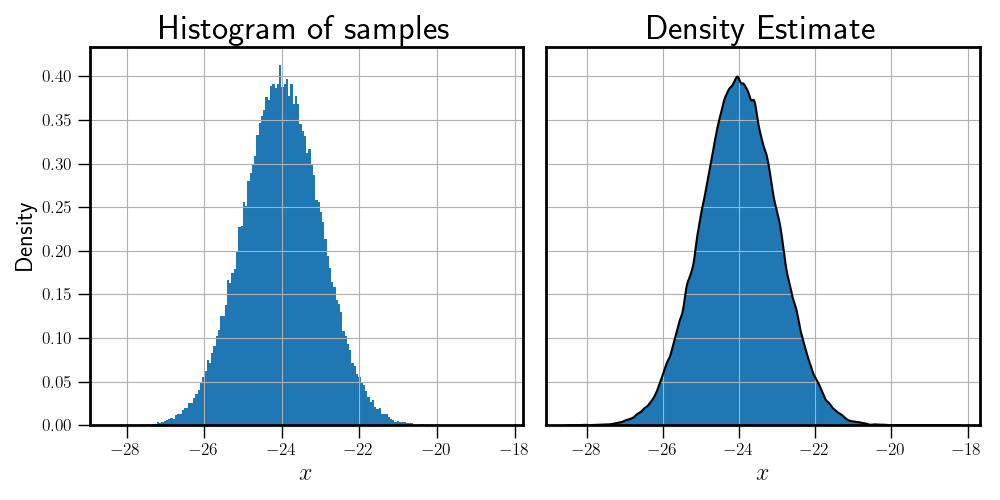
\includegraphics[width=\textwidth]{../Figures/kde_example.png}
        \end{figure}
    \end{frame}

    \begin{frame}
        \frametitle{Kullback-Leibler Divergence - Measuring Entropy Flow}
        Should any given training cause the machine to converge to a fixed state, then for each layer
        we should have that
        \begin{equation}
            {\bf W}_{l,\mathcal{E}}^{(n)}, {\bf W}_{l,\mathcal{D}}^{(n)} \to 
            {\bf W}_{l,\mathcal{E}}^{*}, {\bf W}_{l,\mathcal{D}}^{*} \text{ as }
            n \to \infty \label{eqn:weight convergence}
        \end{equation}
        Consequently, we can charaterize any set of weights via the formulas
        \begin{equation}
            {\bf W}_{l,\mathcal{E}}^{(n)} = {\bf W}_{l,\mathcal{E}}^{*} + {\bf W}_{l,\mathcal{E}}^{(n),f},\
            {\bf W}_{l,\mathcal{D}}^{(n)} = {\bf W}_{l,\mathcal{D}}^{*} + {\bf W}_{l,\mathcal{D}}^{(n),f},
        \end{equation}
        where ${\bf W}_{l,\mathcal{E}}^{(n),f}$ and 
        ${\bf W}_{l,\mathcal{D}}^{(n),f}$ can be thought of as fluctuations from the 
        steady state. Using first-order differencing, we can study the affliated 
        detrended matrices $\delta{\bf W}_{l,\mathcal{E}}^{(n)}$ where
        \begin{align*}
            \delta{\bf W}_{l,\mathcal{E}}^{(n)} &= {\bf W}_{l,\mathcal{E}}^{(n+1)} - {\bf W}_{l,\mathcal{E}}^{(n)} \\
            &= {\bf W}_{l,\mathcal{E}}^{(n+1),f} - {\bf W}_{l,\mathcal{E}}^{(n),f}
        \end{align*}
    \end{frame}

    \begin{frame}
        \frametitle{Kullback-Leibler Divergence - Consecutive Distributions}
        We can consider 
        $\delta{\bf W}_{l,\mathcal{E}}^{(n)}$ to be the deviation from the steady state and with it 
        in hand we flatten it's data and use KDE to generate an affliated empirical probability 
        distribution $p_{l,\mathcal{E}}^{(n)}(w)$. With these distributions we now find the KLD 
        between consecutive distributions to generate the following sequence: 
        \begin{equation}
            D = \bracks{D_{KL}\parens{p_{l,\mathcal{E}}^{(n+1)} \Big|\!\Big| p_{l,\mathcal{E}}^{(n)}}}_{n=1}^{N_E - 2}
        \end{equation}
        which we can interpret to be the change in information between consecutive fluctuations from the 
        steady state.
    \end{frame}

    \begin{frame}
        \frametitle{Kullback-Leibler Divergence - Implementation details}
        After the training of each model for $N_E$ epochs, the 
        data that we have to play with is 
        \begin{equation}
            {\bf W}_\mathcal{E} = \bracks{{\bf W}_{l,\mathcal{E}}^{(n)}}_{n=1, l=1}^{N_E, N_L}, 
            {\bf W}_\mathcal{D} = \bracks{{\bf W}_{l,\mathcal{D}}^{(n)}}_{n=1, l=1}^{N_E, N_L}, 
        \end{equation}
        which are the sets of weights of the layers of the encoder and decoder. Note that both sub-networks 
        have the same number of layers $N_L$ and only differ by the dimension of their inputs and outputs.
        The following procedures are identical for both sets, so we only reference the encoder set
        from here on out. For each layer $l$, the set of detrended matrices are computed
        \begin{equation}
            \delta{\bf W}_{l, \mathcal{E}} = \bracks{{\bf W}_{l,\mathcal{E}}^{(n+1),f} - {\bf W}_{l,\mathcal{E}}^{(n),f}}_{n=1}^{N_E-1},
        \end{equation}
        these matrices are flattened and their entries are used as the data for KDE.
    \end{frame}

    \begin{frame}
        \frametitle{Kullback-Leibler Divergence - Implementation details cont.}
        The kernel used is the Epanechnikov kernel, defined as 
        \begin{equation}
            K(x) = 
            \begin{cases}
                \frac{3(1-x^2)}{4}, & \abs{x} < 1 \\
                0, & \abs{x} \geq 1
            \end{cases},\label{eqn:epanechnikov}
        \end{equation}
        which is optimal in the mean-square error sense. From this, we obtain the set of density estimates for each detrended 
        matrix
        \begin{equation}
            p_{l,\mathcal{E}} = \text{KDE}(\delta{\bf W}_{l, \mathcal{E}}) = \bracks{p_{l,\mathcal{E}}^{(n)}(w)}_{n=1}^{N_E-1}
        \end{equation}
        where $w$ is the weight value itself and $p_{l,\mathcal{E}}(w)$ is the approximate density associated 
        with that weight value. Given these density approximations, we 
        can now compute what we are truly interested in:
        \begin{equation}
            D_l = \bracks{D_{SKL}\parens{p_{l,\mathcal{E}}^{(n+1)} \Big|\!\Big| p_{l,\mathcal{E}}^{(n)}}}_{n=1}^{N_E-2}
        \end{equation}
        Unlike in the first mention, we instead use the SKLD instead of the KLD.
    \end{frame}

    \begin{frame}
        \frametitle{Kullback-Leibler Divergence - Implementation details cont.}
        We are interested in what these divergences tell us about information flow in the model's weights and 
        seek to identify specific classifiers of good training. 
        Can we find quantifiable attributes of the network that behave one way for good training and in a 
        distinguishably different way for bad training? Finding fittings of the data of the divergence data
        is the most reasonable place to start and trends will provide for easier classification. Any overall trend
        is more important to our analysis than lone data points, so to avoid transient behavior skewing any fittings
        we ignore the first 20\% of the divergences computed. We attempt a linear fit on the base 10 logarithm of the data. This 
        corresponds to an exponential fit in the original domain of the divergences with slope of the linear trend 
        being the approximate growth/decay rate of the information flow from the machines steady state. 
        In the interest of trying to find a 
        classifier of good training, we compute the average and variance of the slopes of the linear fits of 
        the layer's divergence data.
    \end{frame}

    \begin{frame}
        \frametitle{Kullback-Leibler Divergence - Example fitting}
        \begin{figure}
            \centering
            \includegraphics[width=\textwidth]{"Z:/ML_models/DLDMD-newest/examples/van_der_pol/trained_models/van_der_pol_07_2022-07-17-1837/div_plot_linear_enc_1"}
        \end{figure}
    \end{frame}

    \begin{frame}
        \frametitle{Results - Duffing}
        \begin{figure}
            \centering
            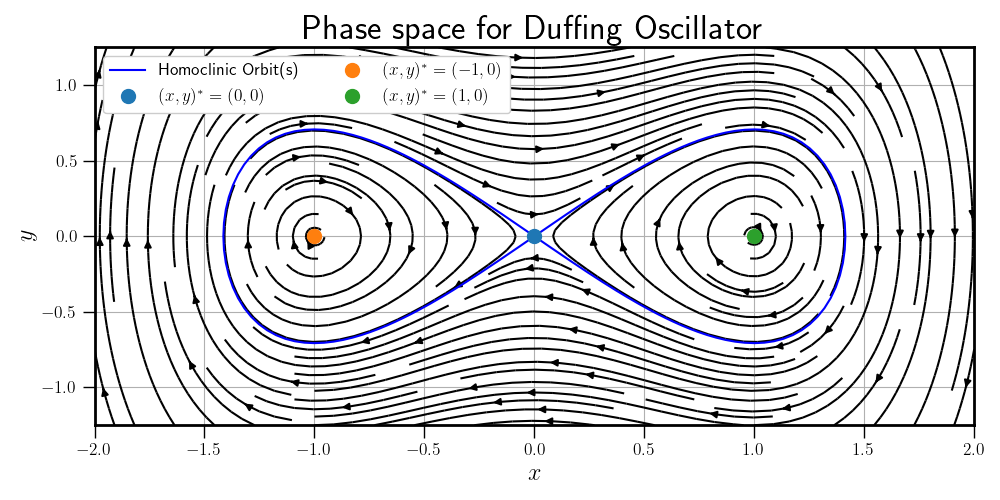
\includegraphics[width=\textwidth]{../Figures/duffing_phase_space.png}
        \end{figure}
    \end{frame}

    \begin{frame}
        \frametitle{Results - Duffing loss curves and phase space}
        \begin{figure}
            \centering
            \begin{minipage}{.5\textwidth}
                \includegraphics[width=\textwidth]{"Z:/ML_models/DLDMD-newest/examples/duffing/loss_plots_square.png"}
            \end{minipage}%
            \begin{minipage}{.5\textwidth}
                \includegraphics[width=\textwidth]{"Z:/ML_models/DLDMD-newest/examples/duffing/experiment_trajectories.png"}
            \end{minipage}
        \end{figure}
    \end{frame}
    
    \begin{frame}
        \frametitle{Results - Duffing linear fit slopes}
        \begin{figure}
            \centering
            \begin{minipage}{.3333\textwidth}
                \includegraphics[width=\textwidth]{"Z:/ML_models/DLDMD-newest/examples/duffing/slope_linear_fit_enc_in_square.png"}
                \includegraphics[width=\textwidth]{"Z:/ML_models/DLDMD-newest/examples/duffing/slope_linear_fit_enc_2_square.png"}
                \includegraphics[width=\textwidth]{"Z:/ML_models/DLDMD-newest/examples/duffing/slope_linear_fit_dec_0_square.png"}
            \end{minipage}%
            \begin{minipage}{.3333\textwidth}
                \includegraphics[width=\textwidth]{"Z:/ML_models/DLDMD-newest/examples/duffing/slope_linear_fit_enc_0_square.png"}
                \includegraphics[width=\textwidth]{"Z:/ML_models/DLDMD-newest/examples/duffing/slope_linear_fit_enc_out_square.png"}
                \includegraphics[width=\textwidth]{"Z:/ML_models/DLDMD-newest/examples/duffing/slope_linear_fit_dec_1_square.png"}
            \end{minipage}%
            \begin{minipage}{.3333\textwidth}
                \includegraphics[width=\textwidth]{"Z:/ML_models/DLDMD-newest/examples/duffing/slope_linear_fit_enc_1_square.png"}
                \includegraphics[width=\textwidth]{"Z:/ML_models/DLDMD-newest/examples/duffing/slope_linear_fit_dec_in_square.png"}
                \includegraphics[width=\textwidth]{"Z:/ML_models/DLDMD-newest/examples/duffing/slope_linear_fit_dec_2_square.png"}
            \end{minipage}
            \includegraphics[width=.3333\textwidth]{"Z:/ML_models/DLDMD-newest/examples/duffing/slope_linear_fit_dec_out_square.png"}
        \end{figure}
    \end{frame}

    \begin{frame}
        \frametitle{Results - Duffing linear fit slope averages and variances}
        \begin{figure}
            \centering
            \includegraphics[width=\textwidth]{"Z:/ML_models/DLDMD-newest/examples/duffing/slope_linear_fit.png"}
        \end{figure}
    \end{frame}

    \begin{frame}
        \frametitle{Results - Duffing notes}

    \end{frame}

    \begin{frame}
        \frametitle{Results - Van der Pol}
        \begin{figure}
            \centering
            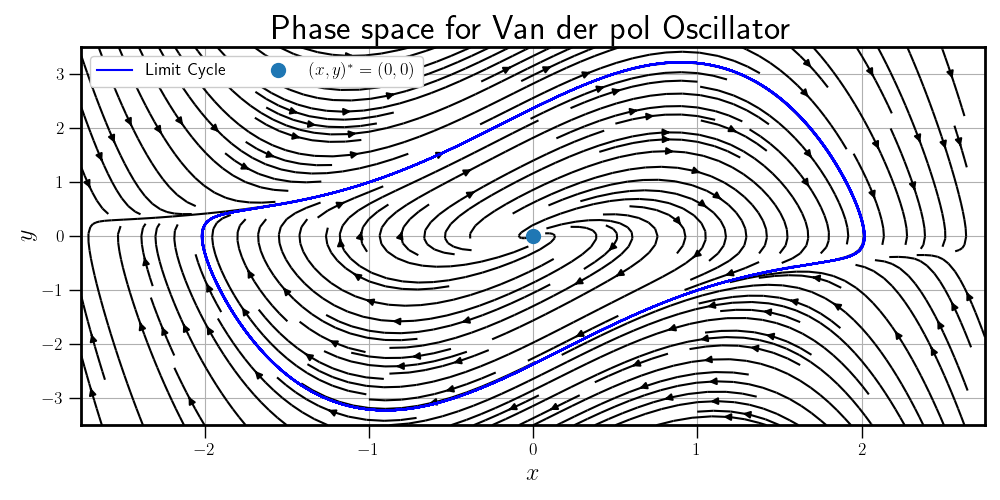
\includegraphics[width=\textwidth]{../Figures/van_der_pol_phase_space.png}
        \end{figure}
    \end{frame}

    \begin{frame}
        \frametitle{Results - Van der Pol loss curves and phase space}
        \begin{figure}
            \centering
            \begin{minipage}{.5\textwidth}
                \includegraphics[width=\textwidth]{"Z:/ML_models/DLDMD-newest/examples/van_der_pol/loss_plots_square.png"}
            \end{minipage}%
            \begin{minipage}{.5\textwidth}
                \includegraphics[width=\textwidth]{"Z:/ML_models/DLDMD-newest/examples/van_der_pol/experiment_trajectories.png"}
            \end{minipage}
        \end{figure}
    \end{frame}

    \begin{frame}
        \frametitle{Results - Van der Pol linear fit slopes} 
        \begin{figure}
            \centering
            \begin{minipage}{.3333\textwidth}
                \includegraphics[width=\textwidth]{"Z:/ML_models/DLDMD-newest/examples/van_der_pol/slope_linear_fit_enc_in_square.png"}
                \includegraphics[width=\textwidth]{"Z:/ML_models/DLDMD-newest/examples/van_der_pol/slope_linear_fit_enc_2_square.png"}
                \includegraphics[width=\textwidth]{"Z:/ML_models/DLDMD-newest/examples/van_der_pol/slope_linear_fit_dec_0_square.png"}
            \end{minipage}%
            \begin{minipage}{.3333\textwidth}
                \includegraphics[width=\textwidth]{"Z:/ML_models/DLDMD-newest/examples/van_der_pol/slope_linear_fit_enc_0_square.png"}
                \includegraphics[width=\textwidth]{"Z:/ML_models/DLDMD-newest/examples/van_der_pol/slope_linear_fit_enc_out_square.png"}
                \includegraphics[width=\textwidth]{"Z:/ML_models/DLDMD-newest/examples/van_der_pol/slope_linear_fit_dec_1_square.png"}
            \end{minipage}%
            \begin{minipage}{.3333\textwidth}
                \includegraphics[width=\textwidth]{"Z:/ML_models/DLDMD-newest/examples/van_der_pol/slope_linear_fit_enc_1_square.png"}
                \includegraphics[width=\textwidth]{"Z:/ML_models/DLDMD-newest/examples/van_der_pol/slope_linear_fit_dec_in_square.png"}
                \includegraphics[width=\textwidth]{"Z:/ML_models/DLDMD-newest/examples/van_der_pol/slope_linear_fit_dec_2_square.png"}
            \end{minipage}
            \includegraphics[width=.3333\textwidth]{"Z:/ML_models/DLDMD-newest/examples/van_der_pol/slope_linear_fit_dec_out_square.png"}
        \end{figure}
    \end{frame}

    \begin{frame}
        \frametitle{Results - Van der Pol linear fit slope averages and variances}
        
        \begin{figure}
            \centering
            \includegraphics[width=\textwidth]{"Z:/ML_models/DLDMD-newest/examples/van_der_pol/slope_linear_fit.png"}
        \end{figure}
    \end{frame}

    \begin{frame}
        \frametitle{Results - Van der Pol notes}

    \end{frame}

    \begin{frame}
        \frametitle{Discussion}

    \end{frame}


    \begin{frame}
        \frametitle{References}
        \bibliographystyle{plain}
        {\footnotesize \bibliography{../main.bib}}
    \end{frame}

    \begin{frame}
        \frametitle{The End!}
        \begin{center}
            \LARGE{Thank you for your time!} \\
            \LARGE{Questions?}
        \end{center}
    \end{frame}
\end{document}